\documentclass[convert]{standalone}

\usepackage{tikz}
\usepackage{graphicx}
\pagestyle{empty}

% INT_AY22_L28-Fig03_g_field_loop.png

\begin{document}
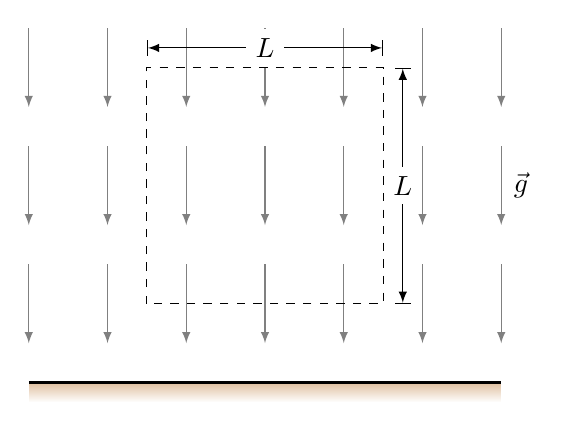
\begin{tikzpicture}[> = latex]

	% Ground
	
	\draw [top color = brown!50, bottom color = white, draw = white] (-3, 0) rectangle (3, -0.25);
	\draw [thick] (-3, 0) -- (3, 0);
	
	% Gravitational field
	
	\foreach \x in {-3, -2, ..., 3}
	\foreach \y in {1.5, 3, 4.5}
		\draw [gray, ->] (\x, \y) -- (\x, \y - 1);
		
	\node at (3.25, 2.5) {${\vec g}$};
		
	% Loop w distance indicators
	
	\draw [dashed] (-1.5, 1) -- (-1.5, 4) -- (1.5, 4) -- (1.5, 1) -- cycle;
	
	\draw [|<->|] (1.75, 1) -- node [fill = white] {$L$} (1.75, 4);
	\draw [|<->|] (-1.5, 4.25) -- node [fill = white] {$L$} (1.5, 4.25);

\end{tikzpicture}
\end{document}